\chapter{Introduction}
\label{chap:intro}

In the early 1990s it was suggested that linguistics might be the first academic discipline to preside over its own demise. As much as 90\% of the world’s 7,000 languages were predicted to become extinct by the end of the 21st century \citep{krauss_worlds_1992,krauss_keynote--mass_2007,campbell_new_2013}. 
Linguists responded by putting greater emphasis on the documentation and description of under-documented languages, and over the past thirty years this effort has steadily broadened our knowledge of the world's languages. Today the estimate of endangered languages is more conservative \citep{eberhard_ethnologue:2020} but still little data or knowledge is available for thousands of languages. It is critical that these languages be documented and described quickly before they disappear. % without sufficient accessible data.

\begin{figure}[tb]
\centering
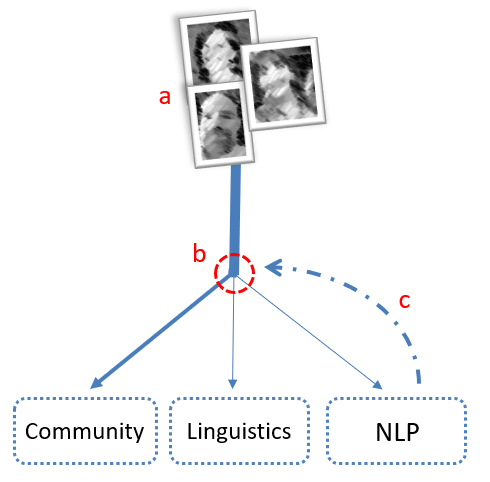
\includegraphics[width=5.75cm]{figs/Flowchart.PNG}
\caption[Language Data Production]{Language Data Production.  A documentary and descriptive field project creates annotated data (a) which can be used for linguistic research, Natural Language Processing (NLP) development, and community efforts to maintain or revitalize the language. Manual annotation has created a bottleneck (b). This dissertation examines methods for integrating NLP into the documentary and descriptive workflow in order to increase annotated language data production (c).}
\label{fig:flowchart}
\end{figure}

The general flow of documentary and descriptive data is illustrated in Figure \ref{fig:flowchart}. A team of linguists and native speakers (a) collaborate to document, conduct basic linguistic analysis, and annotate the documented language data. The annotated data can be used for linguistic research and theory development, the expansion and testing of Natural Language Processing (NLP) algorithms, and for the benefit of the community of speakers who may wish to maintain or revitalize the language. However, because annotation is time- and labor-intensive work, a significant portion of documented language data is bottlenecked and, therefore, inaccessible or difficult to use (b) for linguistic or NLP research and, to a lesser extent, community language development. The methods presented in this dissertation will make more data accessible by integrating NLP machine learning systems into the documentary and descriptive workflow in order to speed and improve the process (c).

Unfortunately, current methods in language documentation and description, especially the process of annotating transcribed texts and analyzing morphological paradigms, are too slow to counteract the crisis of language endangerment. For example, it can take up to 100 hours to manually transcribe a single hour of recorded speech \citep{seifart_language_2018}.
If the process is to match the pace of language extinction, computational methods must be integrated effectively into the workflow of language documentation and description. 

Natural language processing (NLP) did not respond as quickly as linguists to the language endangerment crisis. Although machine learning systems, capable of learning complex patterns in data, have gained tremendous success since the 1990s, NLP research has been focused on a handful of economically or politically powerful languages such as Chinese, Arabic, English, and other European languages. These languages are well documented and described. None 
%demonstrate complicated morphology polysynthetic type, none are under-documented, none 
are endangered.

Fortunately, this is changing. In recent years, NLP research with limited data has burgeoned. This is evidenced, for instance, by the 2015-2019 DARPA-funded Low Resource Languages for Emerging Incidents (LORELEI) project that was motivated in part by the 2014 Haiti earthquake where disaster aid was hampered by the lack of data in Haitian Creole, which is spoken widely in the country, but linguistic resources are so limited, it is rarely encountered in language technology. When Haitian Creole speakers went to social media to cry for help, foreign aid workers struggled to process the information and to inform victims when and where medicine and supplies were available.

Despite this growth, very few NLP systems have been integrated into the process of documenting and describing endangered languages. This lack of integration is largely because state-of-the-art supervised machine learning models depend on large amounts of annotated data (on the order of hundreds of thousands or millions and more tokens), but another challenge to integration is presented by the noise in data created during documentary and descriptive field data. The dynamic, evolving nature of ongoing linguistic analysis during fieldwork and the reliance on manual annotation means that field data is peppered with inconsistencies and typos. To overcome these challenges, methods must be developed that allow documentary and descriptive linguists to benefit from NLP machine learning and \textit{vice versa}.
%Typically, state-of-the-art systems, specifically neural networks, require hundreds of thousands, or even millions, of data instances (words, sounds, sentences, etc.) to achieve state-of-the-art results. Few languages have more than a couple of thousand tokens,
%, let alone much available data, %\mans{The big data requirement is pretty specific to neural models.} 

This dissertation investigates methods for more effectively leveraging machine learning systems for language documentation and description, particularly for morphological analysis and annotation. The research looks at ways that linguists and NLP scientists may want to adjust their expectations and workflows so that both fields can achieve optimal results when working with limited data. 

%\section{Overview of Research}

The overarching question this dissertation asks is \emph{How might the integration of machine learning into language documentation and description affect currently accepted expectations, methods, and workflows?} It addresses that question by examining how current expectations and methods affect machine learning performance on morphological analysis and annotation and exploring new methods for effectively exploiting existing resources to boost machine learning performance on these tasks. This will be done with three studies using various NLP machine learning models and documentary and descriptive corpora from nine under-documented languages. The three studies ask their own specific questions:

\begin{figure}[!b]
    \centering
    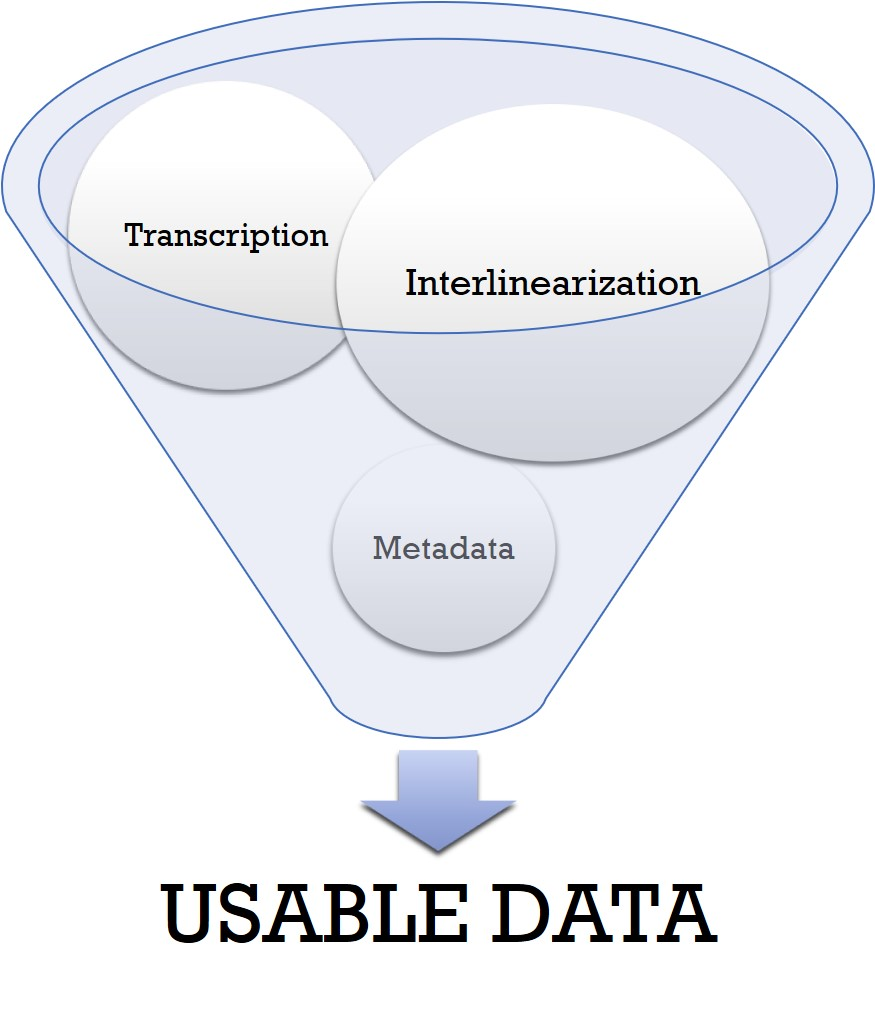
\includegraphics[width=5.5cm]{figs/AnnotationFunnel.jpg}
    \caption[Annotation Bottleneck]{The annotation bottleneck in language documentation and description hinders linguists and NLP scientists from using new language data for research.}
    \label{fig:bottleneck}
\end{figure}


\begin{enumerate}
\item{} \emph{Automating Segmentation and Glossing:} How do variations of research design for morpheme segmentation and glossing which arise from differing conventional expectations in NLP and linguistics affect machine learning performance on those tasks on documentary and descriptive data? 

\item{} \emph{Morphological Paradigm Induction from Interlinear Glossed Texts (IGT2P):} To what extent can machine learning models learn morphological inflection patterns from manually interlinearized texts? Can a human-in-the-loop approach improve results and overcome the inherent noisiness of field data?

\item \emph{Priority of Part of Speech Tagging:} 
What impact does NLP's traditionally high priority on part of speech tagging have on the ability of machine learning systems to perform accurate morpheme segmentation, morpheme glossing, and paradigm induction?
\end{enumerate}

This work is motivated by the “yawning gap” between the amount of documented data deposited in language archives and the portion of the data that is usable for research \citep{seifart_language_2018}. This gap is caused by what has been described as an ``annotation bottleneck'' (Figure \ref{fig:bottleneck}). Current tedious, time-consuming, and expensive annotation tasks are performed primarily by hand from start to finish \citep{simons_worlds_2013,holton_developing_2017}. Manual annotation is subject to human error, introducing inconsistencies and typos, due often not to the difficulty of the task, but to its repetitive and monotonous nature. Other noise in the annotation arises because annotation is also the tool for linguists to begin discovering a language's structure. As linguists' understanding grows, analyses change. These changes are reflected in later annotations, but often not ``corrected'' in earlier annotations.
Budget and time constraints often mean that substantial portions of the data produced by field projects are left uncorrected or simply unannotated. The unannotated portions of documentary corpora remain untapped resources that could inform the development of linguistic science and NLP. They could also support human language technology that would benefit the communities that speak the languages. 

The contributions of this dissertation are four-fold. First, it shows that it is possible and practical to use machine learning to perform morphological annotation by developing and applying methods that improve results on typologically diverse languages with limited training data. Second, by learning inflectional paradigms and accurately generating inflected forms, it demonstrates that machine learning can be used to build and test hypotheses about a language's morphological structure. Third, by training on noisy linguistic field data rather than the curated and polished data that NLP systems are typically trained on, it proves that documentary and descriptive field data, which sometimes the only annotated data available for an under-documented language, can be used to effectively train machine learning models. 
%As such, it may uncover as-yet unforeseen challenges for NLP systems in low-resource settings. 
%It will study what happens when NLP priorities are borrowed directly for documentary and descriptive linguistics, specifically the priority of part of speech (POS) tagging. 
Fourth, it increases annotated data in several low-resource languages which represent a range of field projects, typological structures, and language families. Increased annotated data will allow more thorough testing of linguistic theories and computational models.
Finally, this work presents how new computational methods can be successfully integrated into language documentation and description. 

%\section{Organization}

%%%%%%%%%%%%%%
The rest of the dissertation is organized as follows. Chapter \ref{chap:litreview} provides a background on the linguistic and computational linguistics history and concepts important to this research.
%; it is an expanded version of a paper submitted to \textit{Colorado Research in Linguistics} (CRiL)
Chapter \ref{chap:datamodels} introduces the nine languages and their corpora used in the research and describes the machine learning systems that are implemented in the experiments.
Chapter \ref{chap:seggloss} describes computational methods for segmenting and glossing morphemes and is an expanded version of \citet{moeller_automatic_2018} and \citet{moeller_integrating_2021}. Chapter \ref{chap:IGT2P} describes methods for inducing morphological paradigms from interlinear text and is an expanded version of \citet{moeller_igt2p_2020}. Chapter \ref{chap:POS} looks at the role of part-of-speech (POS) tags for both tasks and is an expanded version of a paper under review at the \textit{North American Chapter of the Association for Computational Linguistics} (NAACL 2021). Finally, Chapter \ref{chap:conclusion} summarizes the impacts of this research and outlines work that could build upon this research and further integrate machine learning into language documentation and description.